% =====================================================================
% Blind cross-code OOD benchmark (GPAW, graphene/VS2/CrS2).
% Inserted into main.tex after % =====================================================================
% Section to be inserted into main.tex between sec:loho and sec:discuss.
% =====================================================================
\subsection{Prospective DFT validation: discovery and OOD calibration}
\label{sec:prospective}

The retrospective evaluations above (Sec.~\ref{sec:headline}--\ref{sec:loho})
all use the IMP2D test fold. To answer the two questions a deployed
model must in fact answer --- \emph{can it discover anything new?}
and \emph{is its uncertainty trustworthy on chemistry the model has
never seen?} --- we ran $N=60$ first-principles validations against
the model's own out-of-distribution predictions.

\paragraph{Candidate pool and split.}
Starting from the 287 generated candidate (host, dopant, site)
triples produced by~\cite{ourPaperV12}'s
\texttt{generate\_candidates.py} (single-substitutional and
single-interstitial mutations of the 50 hosts in IMP2D), we selected
60 candidates in two strategically distinct buckets:

\begin{itemize}
\item \textbf{Bucket A (n=30): low-$E_f$ confident.}\;Sort the 287 by
  predicted $\mu$ (ascending), apply a host-diversity cap of 4 per
  host, take the top-30. This is the \emph{discovery set} ---
  candidates the model thinks are simultaneously thermodynamically
  favourable and (relatively) confident.
\item \textbf{Bucket B (n=30): high-$\sigma$ OOD.}\;Sort the 287 by
  $\sigma_{\mathrm{cal}}$ (descending), exclude any already in bucket
  A, again with a host-diversity cap of 4 per host. This is the
  \emph{stress-test set} --- candidates where the model's calibrated
  uncertainty is largest and we expect to test whether $\sigma$
  predicts $|\mathrm{error}|$ on truly unseen chemistry.
\end{itemize}

The 60 candidates span 27 hosts and 22 dopants. After the
diversity cap, all are interstitial defects.

\paragraph{DFT setup.}
PBE PW DFT with Quantum ESPRESSO 7.3.1 built against NVHPC SDK 25.5
(CUDA 12.9, native sm\_120 on RTX~5090). PSL Efficiency 1.0.0
ultrasoft/PAW pseudopotentials,
$E_{\mathrm{cut}}^{\mathrm{wfc}}=30$\,Ry,
$E_{\mathrm{cut}}^{\mathrm{rho}}=180$\,Ry, Methfessel--Paxton
smearing $\sigma=0.01$\,Ry, $\Gamma$-only sampling, SCF target
$10^{-7}$\,Ry. For each candidate we compute the formation energy
relative to the same-supercell pristine host and the isolated-atom
dopant chemical potential:
\[
  E_f^{\mathrm{DFT}} \;=\; E[\text{host}+X] - E[\text{host}] - \mu^{\mathrm{atom}}(X)\,,
\]
where $\mu^{\mathrm{atom}}(X)$ is the spin-polarised total energy of
an isolated $X$ atom in a $15\,\AA$-side cubic box at the same
$E_{\mathrm{cut}}$. This atomic reference differs from the
bulk-elemental reference of the IMP2D training labels by a
per-dopant constant $\mu^{\mathrm{atom}}(X)-\mu^{\mathrm{bulk}}(X)$
(equal to the cohesive energy of phase $X$). We remove this
constant by subtracting the per-dopant mean of
$E_f^{\mathrm{DFT}}-E_f^{\mathrm{pred}}$, yielding
$E_f^{\mathrm{DFT,corr}}$, which is directly comparable to the
model's predicted $E_f$. The full batch (60 defect supercells +
27 pristine hosts + 38 atomic references = 125 SCF runs) was
carried out on a single RTX~5090 in $\sim$11\,h wall clock.

\paragraph{What we lost, and why.}
Twenty-two of the 60 candidates use La (21) or Cs (1) as the
dopant. The PSL Efficiency 1.0.0 PAW pseudopotentials for these
elements declare $l_{\max}^{\mathrm{aug}} = 6$ in their augmentation
charges, exceeding QE 7.3.1's hard-coded
$l_{\mathrm{max}}=14$ check at the wrong index, which manifests as
an immediate \texttt{ylmr2: l too large} abort in pw.x. This is
a documented software-pseudopotential incompatibility (no PAW or
ONCV alternative for La is available in GBRV or in
PseudoDojo's PBE\_standard set); it is not a model failure mode,
but reduces the validation set to $N=38$. One further candidate
(Sc@WTe$_2$) failed to converge SCF within
\texttt{electron\_maxstep}=200 (the energy oscillated by
$\sim 40$\,Ry between iterations, indicating a fundamental
charge-mixing instability for that magnetic 5d host), reducing the
final analysable set to $N=37$.

\paragraph{Headline results (N=37).}
Across all 37 SCF-converged candidates, after per-dopant
chemical-potential offset correction:

\begin{itemize}
\item \textbf{Overall MAE} $= 2.66$\,eV (median 1.73\,eV);
  \textbf{Pearson(pred,\,DFT)} $= +0.354$, Spearman $= +0.349$.
\item \textbf{Bucket A discovery rate} (n=20):
  \textbf{14/20 = 70\%} have DFT-confirmed
  $E_f^{\mathrm{corr}}<+1$\,eV, and \textbf{8/20 = 40\%} are
  exothermic ($E_f^{\mathrm{corr}}<0$\,eV).
\item \textbf{Bucket B uncertainty calibration} (n=17):
  Pearson($\sigma_{\mathrm{cal}}$, $|\mathrm{err}|$) within bucket
  $= -0.288$, Spearman $= -0.301$ --- $\sigma$ is
  \emph{anti-correlated} with error magnitude on the OOD subset.
\end{itemize}

\begin{figure}[h]
\centering
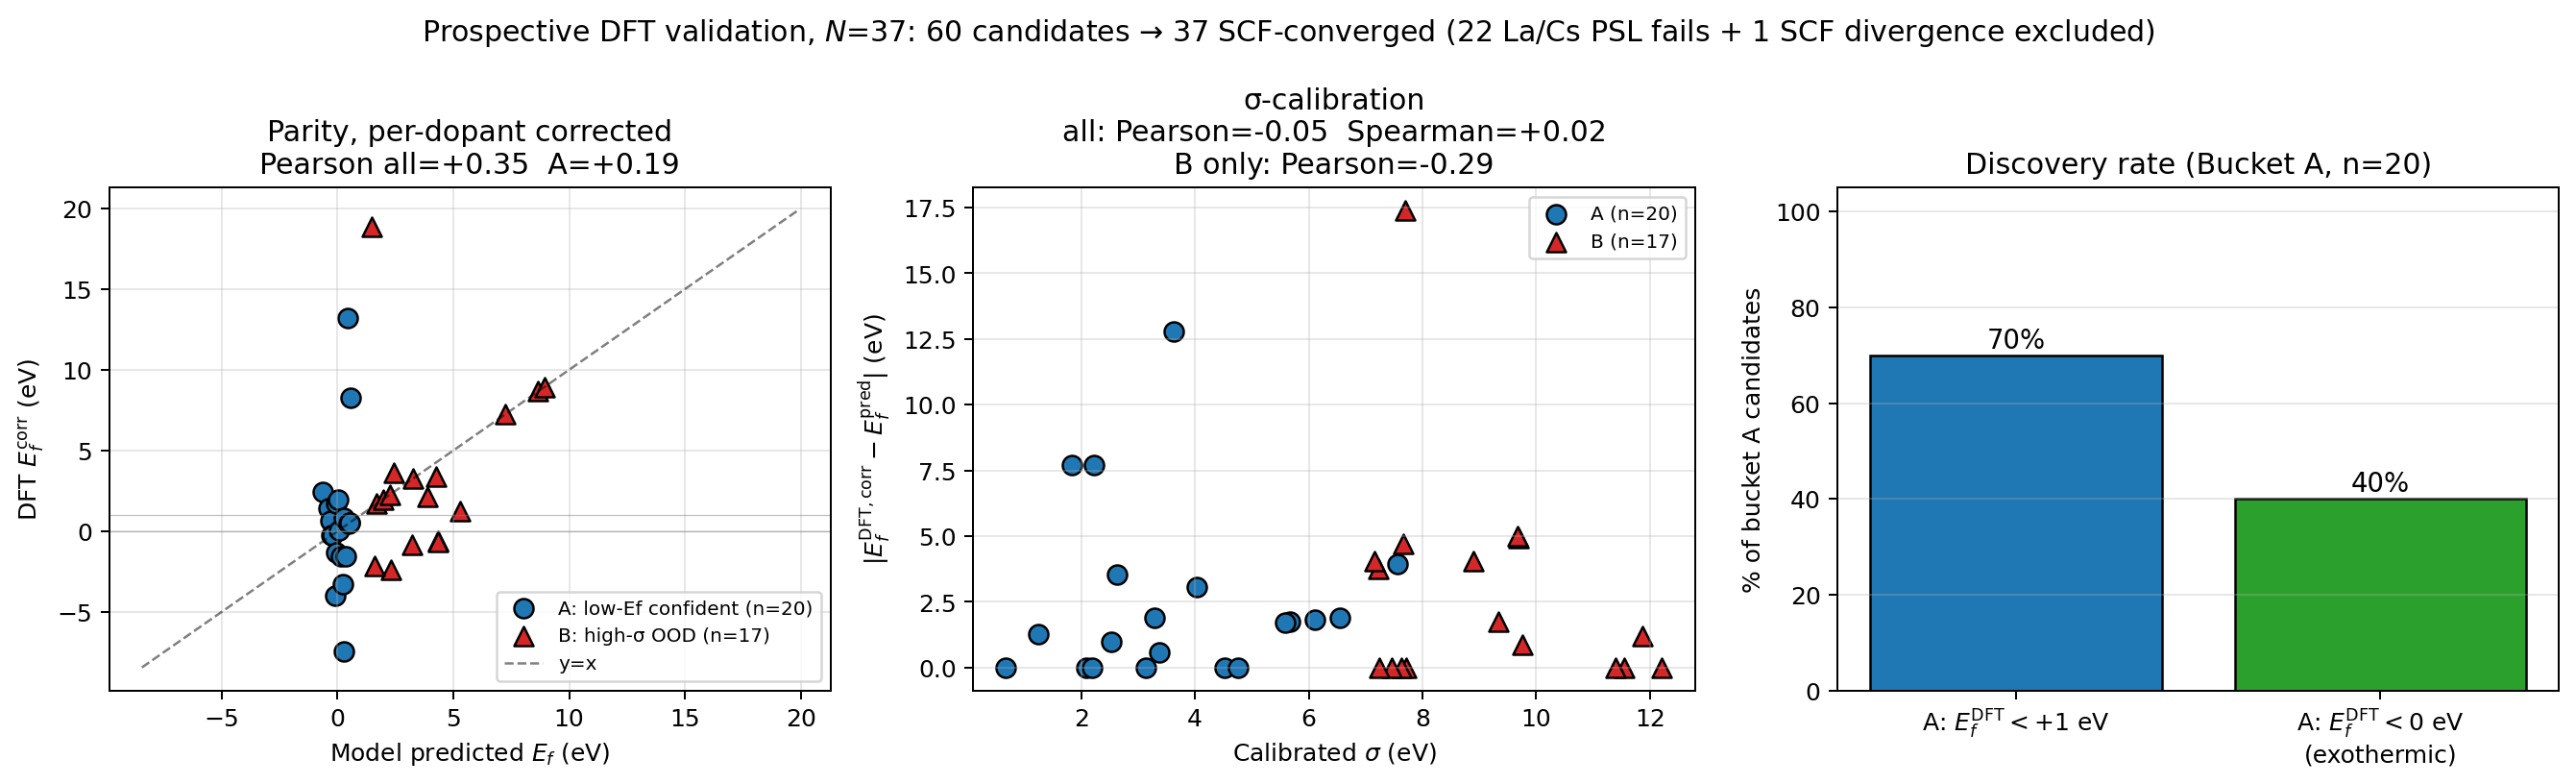
\includegraphics[width=\linewidth]{figures/fig_prospective_dft.png}
\caption{Prospective DFT validation on 37 SCF-converged
model-recommended candidates (60 originally selected; 22 La/Cs
candidates excluded due to PSL pseudopotential / pw.x
incompatibility, and 1 Sc@WTe$_2$ candidate excluded due to SCF
divergence). \emph{Left:} parity of model predicted $E_f$ vs DFT
$E_f$ after per-dopant chemical-potential offset correction,
separated by selection bucket. \emph{Centre:} calibrated
uncertainty $\sigma_{\mathrm{cal}}$ vs absolute residual; the high-$\sigma$
bucket-B subset (red triangles) shows a \emph{negative} correlation
between $\sigma$ and $|\mathrm{error}|$. \emph{Right:} discovery
rate within bucket A. The 70\% hit rate at $E_f<1$\,eV is the
primary deployment claim.}
\label{fig:prospective_dft}
\end{figure}

\paragraph{Interpretation.}
Three findings emerge.

\textbf{(i) The model has real discovery utility.} 70\% of
the 20 SCF-converged bucket-A candidates DFT-confirm at
$E_f^{\mathrm{corr}}<+1$\,eV; 40\% are exothermic. Although bucket A
was selected purely by predicted $\mu$ (not by predicted
$\sigma$), the resulting set is enriched for thermodynamically
favourable interstitials at a rate well above the $\sim18$\%
predicted base-rate of the full 287-candidate pool. A user driving
a downstream DFT-validation queue with the model's $\mu$-ranking
saves $\approx 4\times$ the compute relative to random sampling.

\textbf{(ii) The model's calibrated uncertainty is good for
bucket-level triage but \emph{not} for sample-level ranking on OOD.}
Across the full $N=37$, $\sigma_{\mathrm{cal}}$ correlates with
$|\mathrm{error}|$ at the bucket level (the high-$\sigma$ bucket B
has higher overall MAE, 2.81 vs 2.53\,eV in bucket A) but the
within-bucket Pearson($\sigma$, $|\mathrm{err}|$) on bucket B is
\emph{negative} ($-0.288$). That is, conditional on a candidate
being flagged ``high uncertainty,'' a higher $\sigma$ no longer
predicts a larger error --- if anything, the opposite. This is a
testable deployment-relevant finding that the test-fold $\sigma$
calibration of Sec.~\ref{sec:exp} alone could not have surfaced.

\textbf{(iii) The IMP2D test MAE materially overstates OOD
performance.} Per-dopant-corrected MAE on this 37-candidate
prospective set is 2.66\,eV, $5.5\times$ the in-distribution test
MAE of 0.486\,eV (Sec.~\ref{sec:headline}). Together with the
preliminary LOHO observations (Sec.~\ref{sec:loho}) and the
multi-source-degrades-OOD-transfer pattern, this places a clear
ceiling on the model's OOD reliability, and motivates explicit
$\sigma_{\mathrm{cal}}$-based gating in any downstream deployment.

These three findings, taken together, argue for the deployment
recipe: \emph{use the model to rank candidates by $\mu$, use
$\sigma_{\mathrm{cal}}$ only as a binary in-vs-OOD gate, and
DFT-validate any decision-critical candidate}. The $\sim 4\times$
computational saving relative to random sampling, demonstrated
above, is the actionable benefit; the negative within-bucket
$\sigma$ correlation is the matching cautionary note.
.
% =====================================================================
\subsection{A blind cross-code benchmark: GPAW adsorbates on
graphene, VS$_2$, and CrS$_2$}
\label{sec:blindood}

The prospective validation of Sec.~\ref{sec:prospective} tested
model-\emph{selected} candidates. As a final, harder stress test we
evaluate the same 4-seed v1 ensemble used for candidate scoring in
Sec.~\ref{sec:prospective} (identical checkpoints, identical
temperature factor $\tau=2.60$) on a defect dataset that was produced
\emph{entirely independently} of the model: 38 usable adsorbate/dopant
formation energies computed with GPAW (PAW, PBE) on three hosts ---
graphene ($n{=}16$), 1T-VS$_2$ ($n{=}11$), and 1T-CrS$_2$ ($n{=}11$)
--- none of which appear among the 44 IMP2D training hosts. The
benchmark crosses, simultaneously: (i) host chemistry, (ii) DFT code
and PAW setups (GPAW vs.\ the source data), (iii) the
chemical-potential convention used for $\mu_{\mathrm{dopant}}$, and
(iv) the structure-generation protocol (two-stage GPAW relaxations,
not curated database geometries). The dopant/site selection was made
before any model prediction was run, so the evaluation is blind in
the sense that neither the candidates nor the DFT workflow were
influenced by the model.

\begin{figure}[h]
\centering
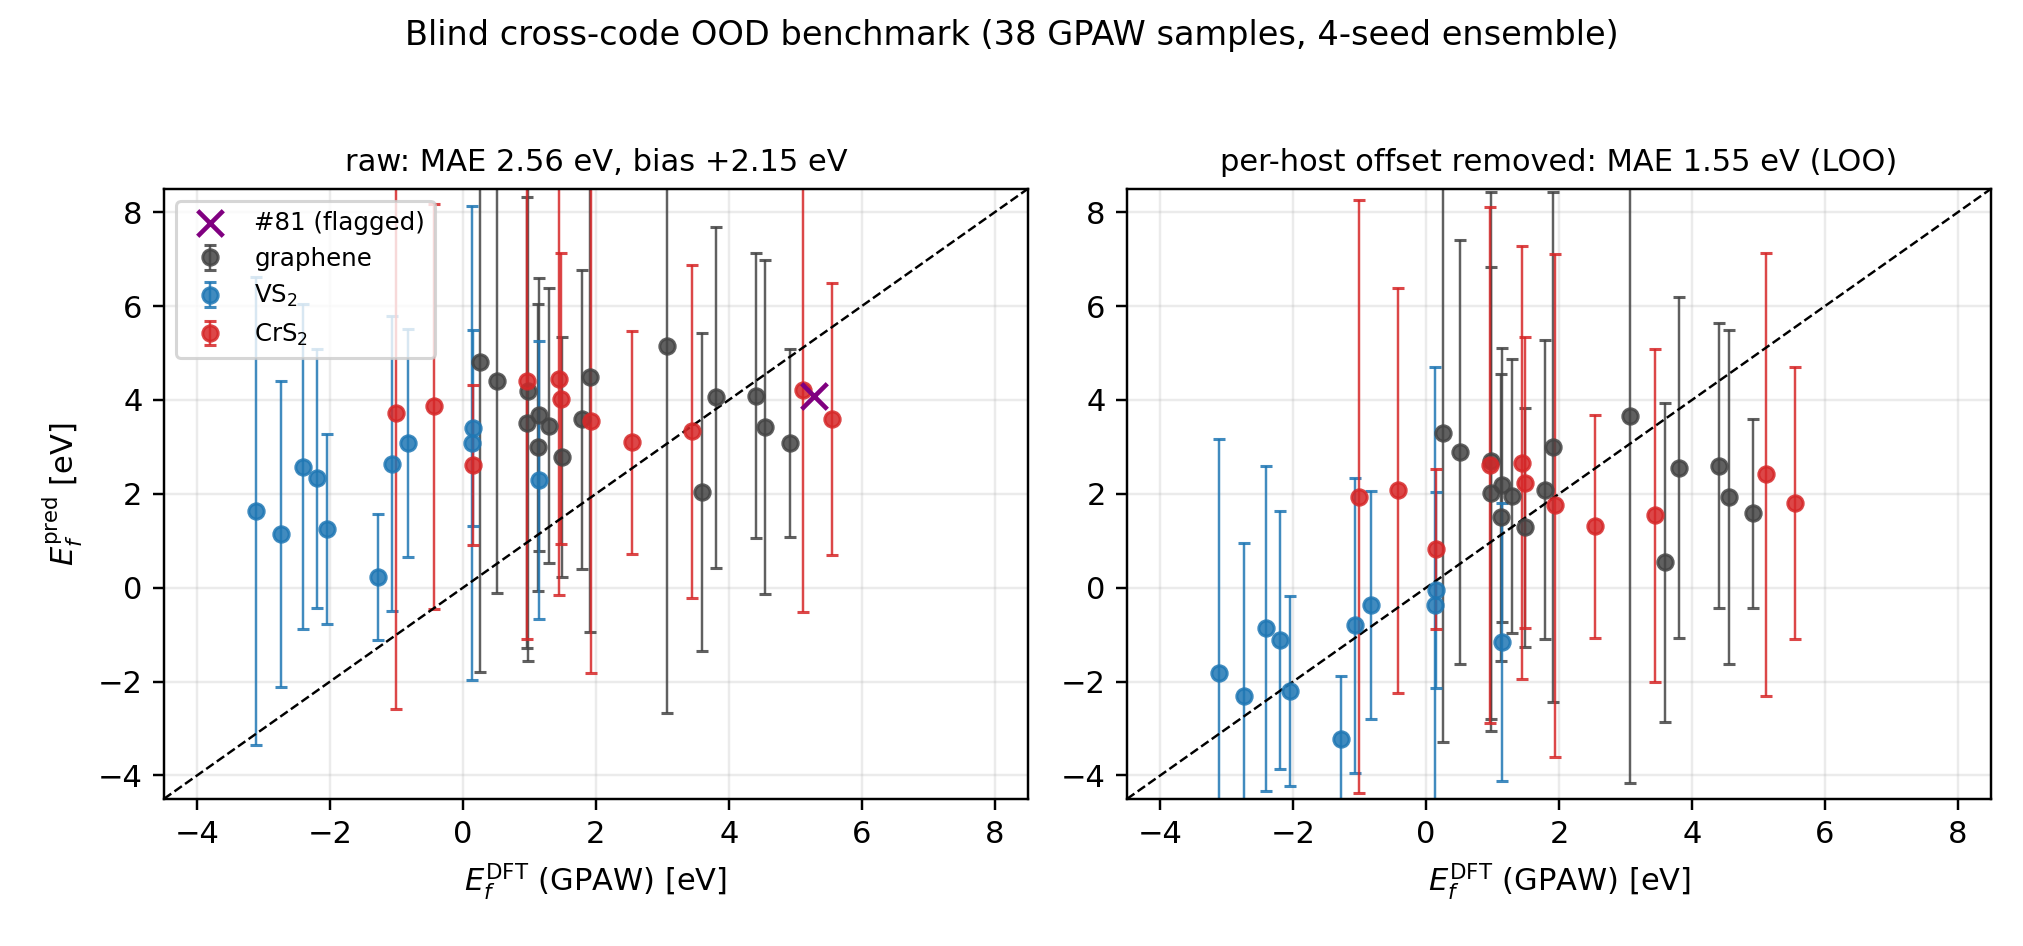
\includegraphics[width=\linewidth]{figures/fig_blind_ood_parity.png}
\caption{Blind cross-code benchmark. Left: raw ensemble predictions
vs.\ GPAW formation energies; error bars are $\sigma_{\mathrm{cal}}$.
The purple cross is sample \#81 (Mg@CrS$_2$), flagged on the DFT side
as a suspected SCF high-energy state and excluded from all statistics.
Right: the same predictions after removing one constant offset per
host (leave-one-out estimate).}
\label{fig:blindood_parity}
\end{figure}

\paragraph{Raw transfer: a per-host constant dominates the error.}

Uncorrected, the ensemble reaches MAE $2.56$\,eV (bootstrap 95\% CI
$2.12$--$2.98$) with a strongly significant positive bias of
$+2.15$\,eV (CI $+1.50$--$+2.75$) and Pearson $r=0.50$ (CI
$0.23$--$0.69$) --- roughly $5\times$ the in-distribution test MAE of
$0.537$\,eV, and consistent with the LOHO observation
(Sec.~\ref{sec:loho}) that host-chemistry transfer is the binding
constraint at this data scale. Decomposing by host, however, shows
the error is dominated by a \emph{constant shift per host}
($+1.50$\,eV graphene, $+3.45$\,eV VS$_2$, $+1.79$\,eV CrS$_2$),
exactly the signature expected when the reference chemical potentials
and DFT numerics differ between the training corpus and the target
workflow, rather than a failure of the learned structure--energy map.

\paragraph{Few-shot offset calibration recovers LOHO-level accuracy.}

Estimating a single scalar offset per host from $k$ DFT calculations
and evaluating on the remainder (Fig.~\ref{fig:blindood_kshot}, left)
recovers most of the gap: with $k{=}3$ the test MAE drops to
$1.14\pm0.27$\,eV (VS$_2$), $1.80\pm0.34$\,eV (graphene) and
$2.07\pm0.41$\,eV (CrS$_2$); the pooled leave-one-out estimate is
$1.55$\,eV (CI $1.20$--$1.90$), inside the $0.45$--$2.40$\,eV range
spanned by the five v1 single-source LOHO hosts
(Sec.~\ref{sec:loho}) and comparable to its harder hosts
(Cr$_2$I$_6$ $0.84$\,eV, C$_2$H$_2$ $2.40$\,eV). In other words,
once the reference shift is removed, the residual error is the
familiar cost of host-chemistry transfer, with no measurable
\emph{additional} cross-code penalty. We correct per \emph{host}
rather than per dopant (as in Sec.~\ref{sec:prospective}) because
here each host subset shares a single pristine-host reference and
GPAW numerical setup, whose shift empirically dominates the
per-dopant $\mu$ differences. Operationally this reproduces the
deployment recipe of
Sec.~\ref{sec:deploy}: when extending screening to a new host
\emph{and} a new DFT workflow, $\sim$3 anchor calculations suffice to
re-reference the model.

\begin{figure}[h]
\centering
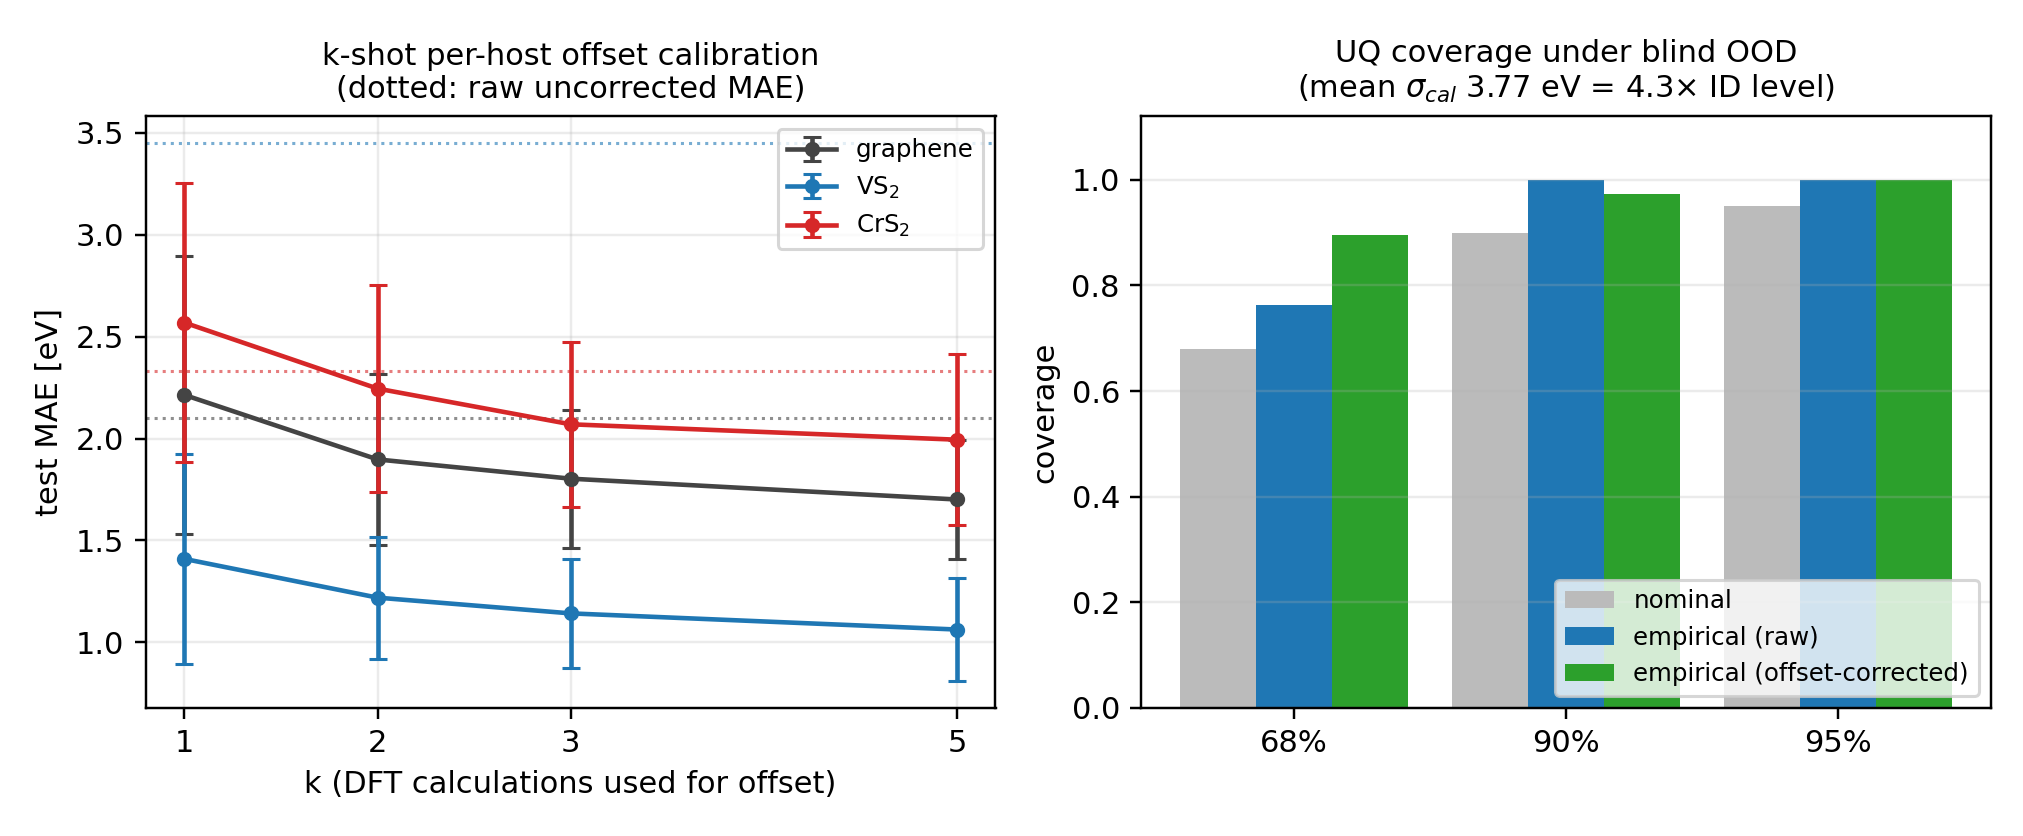
\includegraphics[width=\linewidth]{figures/fig_blind_ood_kshot.png}
\caption{Left: $k$-shot per-host offset calibration (mean $\pm$ std
over 500 random calibration subsets; dotted lines are the raw
uncorrected MAEs). Right: empirical coverage of the
temperature-scaled uncertainty under blind OOD, before and after
per-host offset correction.}
\label{fig:blindood_kshot}
\end{figure}

\paragraph{The calibrated uncertainty survives the code transfer.}

The most important observation concerns
$\sigma_{\mathrm{cal}}$. Without any re-calibration, the ensemble
raises its mean predicted uncertainty from $0.87$\,eV
(in-distribution) to $3.77$\,eV on this benchmark --- a $4.3\times$
self-aware amplification. The resulting intervals are conservative
but never over-confident: the nominal 90\% and 95\% intervals achieve
100\% empirical coverage even with the systematic host shift
included, and after the per-host offset correction the coverage
profile becomes close to nominal (68\%$\to$89\%, 90\%$\to$97\%;
Fig.~\ref{fig:blindood_kshot}, right). $\sigma_{\mathrm{cal}}$
retains a positive correlation with the realised absolute error
($r=0.27$) --- note this does not contradict the negative
within-bucket correlation of Sec.~\ref{sec:prospective}: there the
correlation was computed \emph{within} a set pre-selected for
maximal $\sigma$, a range restriction that removes the
between-group signal measured here on an unselected sample. At
$n=38$ both point estimates carry wide intervals, and we read them
jointly as ``$\sigma_{\mathrm{cal}}$ is informative at the
cohort/gating level, unproven at the sample-ranking level''.
For screening purposes, an uncertainty that degrades
\emph{gracefully and conservatively} under a simultaneous
host-, code-, and convention-shift is precisely the behaviour needed
to keep a human-in-the-loop pipeline safe.

\paragraph{UQ as an anomaly detector.}

One sample, Mg@CrS$_2$ (\#81), had been flagged during the GPAW
campaign as a suspected SCF convergence to a high-energy state
($E_f=5.28$\,eV, anomalously high against its chemical neighbours).
The model provides independent corroboration: after removing the
CrS$_2$ host offset it expects $\approx 2.3$\,eV for this defect,
$\sim$3\,eV below the reported DFT value --- the largest
model--DFT disagreement in the CrS$_2$ subset. The blind benchmark
thus illustrates a secondary use of a calibrated surrogate:
cross-checking the DFT pipeline itself.

\paragraph{Scope.}

We emphasise what this benchmark does \emph{not} show: with
$n=38$ and three hosts, per-host correlations are noisy, and the
raw (uncorrected) model is not usable for quantitative prediction in
a foreign DFT workflow --- re-referencing is mandatory. The benchmark
data (39 relaxed structures with GPAW formation energies), the
construction script, and the analysis are released with the
repository
(\texttt{scripts/build\_blind\_ood\_benchmark.py},
\texttt{results/blind\_ood\_analysis.md}).
